\documentclass[14pt]{beamer}
\usepackage[T2A]{fontenc}
\usepackage[utf8]{inputenc}
\usepackage[english,russian]{babel}
\usepackage{tikz}
\usepackage[european,cuteinductors,smartlabels]{circuitikz}

\usepackage{amssymb,amsfonts,amsmath,mathtext}
\usepackage{amssymb}
\usepackage{cite,enumerate,float,indentfirst}
\usepackage{cancel}
\usepackage{csquotes}
\newcommand{\quotes}[1]{``#1''}

%\usepackage{pgfplots}
%\usepackage[left=1cm,right=1cm, top=1cm,bottom=1cm,bindingoffset=0cm]{geometry}

% Beamer — верстаем презентации  https://habrahabr.ru/post/145523/ 
\graphicspath{{images/}}

\usetheme{Pittsburgh}
\usecolortheme{whale}

\setbeamercolor{footline}{fg=blue}
\setbeamertemplate{footline}{
\leavevmode%
\hbox{%
\begin{beamercolorbox}[wd=.333333\paperwidth,ht=2.25ex,dp=1ex,center]{}%
Прокшин А.Н. и др.
\end{beamercolorbox}%
\begin{beamercolorbox}[wd=.333333\paperwidth,ht=2.25ex,dp=1ex,center]{}%
Санкт-Петербург, 2019
\end{beamercolorbox}%
\begin{beamercolorbox}[wd=.333333\paperwidth,ht=2.25ex,dp=1ex,right]{}%
Стр. \insertframenumber{} из \inserttotalframenumber \hspace*{2ex}
\end{beamercolorbox}}%
\vskip0pt%
}

\newcommand{\itemi}{\item[\checkmark]}

	\usefonttheme[onlymath]{serif} % в формулах использовать текст с засечками
\begin{document}
\title{\small{Создание и апробирование лабораторной установки по учебному курсу Микроконтроллеры по теме \enquote{Генерация векторного ШИМ для управления трехфазным асинхронным двигателем}.}}
\author{\small{%
\emph{авторы:}~Василенко Виктор Андреевич\\%
\emph{}~Вербова Алина\\
\emph{}~Илюшин Антон Геннадьевич\\
\emph{}~Маслов Иван Андреевич\\
\emph{}~Прокшин Артем Николаевич\\% 
\emph{}~Халявин Дмитрий Игоревич}}



\institute{Санкт-Петербургский государственный электротехнический университет «ЛЭТИ» им. В.И. Ульянова (Ленина)}
\vspace{30pt}%
%Санкт-Петербургский государственный электротехнический университет\\
%«ЛЭТИ» им. В.И. Ульянова (Ленина)

\vspace{60pt}%

%\date{\small{Санкт-Петербург, 2019}}

\AtBeginSection{
	\begin{frame}
		\frametitle{Содержание}
		\tableofcontents[currentsection]
	\end{frame}
}

\begin{frame}
\titlepage	
\end{frame}

%\begin{frame}
%        \frametitle{Содержание}
%        \tableofcontents[currentsection] 
%\end{frame}
\begin{frame}
\frametitle{\small Цели, к которым стремились при реализации курса} 
\begin{itemize}
\item упрощение системы управления с использованием ковариантных и контравариантных координат;
\item использование дипломных проектов студентов предыдущих выпусков;
\item создание лабораторных стендов по тематике кафедры с перспективой на использование российских разработок;
\item использование свободного open-source программного обеспечения;
\item оформление УМКД;
\item ... будет сформулирована в результатах.
\end{itemize}
\end{frame}

\begin{frame}
\frametitle{\smallвнутренние ресурсы, на которые опирались}
\begin{itemize}
	\itemНа кафедре есть курсы по управлению приводом с помощью контроллеров ОМРОН; 
	\itemесть дешевые микроконтроллеры(SoC); увеличилась скорость, разрядность, есть функции управления эл.двигателями; 
	\itemпредыдущий курс \enquote{решение интерфейсных задач с помощью микроконтроллера at89} Кекконен А.В.,Тимофеев А.А.,который выполняется на asm,C в ``Keil''(8 установок); 
\itemобсуждалось (приводчикам нужны приводы) с Татаринцевым Н.И., Беловым М.П.;
\itemподелили:Татаринцев --двигатель постоянного тока, Прокшин -- асинхронный двигатель.  
\end{itemize}
\end{frame}


\begin{frame}
\frametitle{\smallпрограммы -- бесплатно}
\begin{itemize}
	\item в ОС Linux всё необходимое присутствует  ``из-коробки'':
		\begin{itemize}
		\item кросс-компилятор arm-none-eabi-gcc
		\item компилятор для ``родной'' системы gcc, g++
		\item  java-1.8.0-openjdk;
		\end{itemize}
	\item эти компиляторы возможно запускать в среде эмуляции Линукс(cygwin) в ОС Windows;
	\item STM выкупила  и сделала Atollic Studio бесплатным
		для своих микроконтроллеров. \href{atollic.com}{Atollic Studio} работает на всех ОС;
	\item www.ac6.fr выпускает бесплатный компилятор \href{www.openstm32.org}{System Workbench} 
на среде Eclipse и работает на всех операционных системах.
\end{itemize}
\end{frame}


\begin{frame}
\frametitle{\smallоборудование -- дешево} 
\begin{figure}
\begin{center}
\begin{minipage}[h]{0.5\linewidth}
\center{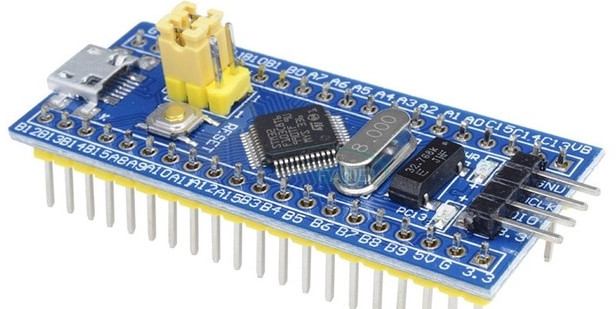
\includegraphics[width=1\linewidth]{stm32f103c8t6.jpg}}  \\
\end{minipage}
\end{center}
\end{figure} 
\begin{tabular}{lll}
	1&микроконтроллер		&200руб.\\
	2&аппаратный программатор	&200-300руб.\\
	3&светодиод,резистор,провода&100руб\\
	4&драйвер силовых ключей&в единственном экз.\\
	5&асинхронный двигатель&в единственном экз.\\
	6&силовой блок питания&в единственном экз.\\
	7&осциллограф&в единственном экз.
\end{tabular}
\end{frame}


\begin{frame}
\frametitle{\smallудача -- не нужен аппаратный программатор}
оказалось, что возможно использовать начальную область памяти самого микроконтроллера для программы-загрузчика. После окончания работы программы-загрузчика управление
передается в область памяти сразу за загрузчиком.
	\vspace{0.5cm}

описание на русском https://habr.com/post/403007/\\
%на английском %http://www.rogerclark.net/stm32f103-and-maple-maple-mini-with-arduino-1-5-x-ide/

	Сама  программа загрузчик -- \\
{\small https://github.com/rogerclarkmelbourne/Arduino\_STM32} 
\end{frame}


\begin{frame}
\frametitle{\smallЛекция 1 Ковариантные координаты изображающего вектора}
$$
        \vec{f} = \frac{2}{3}\left(f_{a_{\!\perp}}\!\vec{e}_a + f_{b_{\!\perp}}\!\vec{e}_b + f_{c_{\!\perp}}\!\vec{e}_c\right)
$$
%
\begin{tabular}{cl}
\begin{minipage}[h]{0.3\linewidth}
\begin{tikzpicture}[scale=2]
\newcommand{\D}){8}
\draw[->, very thin] (0,0) -- (1.00, 0.00);
\draw[->, very thin] (0,0) -- (0.95, 0.31);
\draw[->, very thin] (0,0) -- (0.81, 0.59);
%\draw[->, very thin] (0,0) -- (0.59, 0.81);
\draw[yellow, very thick,->,>=stealth'] (0,0) -- (0.59,0);
\draw[green, very thick,->,>=stealth'] (0,0) -- (-0.20,0.35);
\draw[red, very thick,->,>=stealth'] (0,0) -- (0.50,0.86);
\draw[->,thick] (0,0) -- (0.59, 0.81) node[above right] {$\vec{f}$};
\draw[->, very thin] (0,0) -- (0.31, 0.95);
\draw[->, very thin] (0,0) -- (0.00, 1.00);
\draw[->, very thin] (0,0) -- (-0.31, 0.95);
\draw[->, very thin] (0,0) -- (-0.59, 0.81);
\draw[->, very thin] (0,0) -- (-0.81, 0.59);
\draw[->, very thin] (0,0) -- (-0.95, 0.31);
\draw[->, very thin] (0,0) -- (-1.00, 0.00);
\draw[->, very thin] (0,0) -- (-0.95, -0.31);
\draw[->, very thin] (0,0) -- (-0.81, -0.59);
\draw[->, very thin] (0,0) -- (-0.59, -0.81);
\draw[->, very thin] (0,0) -- (-0.31, -0.95);
\draw[->, very thin] (0,0) -- (-0.00, -1.00);
\draw[->, very thin] (0,0) -- (0.31, -0.95);
\draw[->, very thin] (0,0) -- (0.59, -0.81);
\draw[->, very thin] (0,0) -- (0.81, -0.59);
\draw[->, very thin] (0,0) -- (0.95, -0.31);
\end{tikzpicture} 
\end{minipage}
&
\begin{minipage}[h]{0.7\linewidth}
	{\small\begin{itemize}
\item измеряемые величины -- ковариантные координаты вектора; 
\item физическая величина -- всегда произведение двух ко- и контра-координат;
\item изображающий вектор симметричной системы есть $2/3 (I_a + I_b + I_c)$;
\item рисунок -- есть результат 1й практической работы.
\end{itemize}
	}
\end{minipage}
\end{tabular}
\end{frame}

\begin{frame}
\frametitle{\smallконтравариантные координаты -- управление}

\end{frame}

\begin{frame}
\frametitle{\smallфото установки}
\begin{figure}
\begin{center}
%\begin{minipage}[h]{0.5\linewidth}
\center{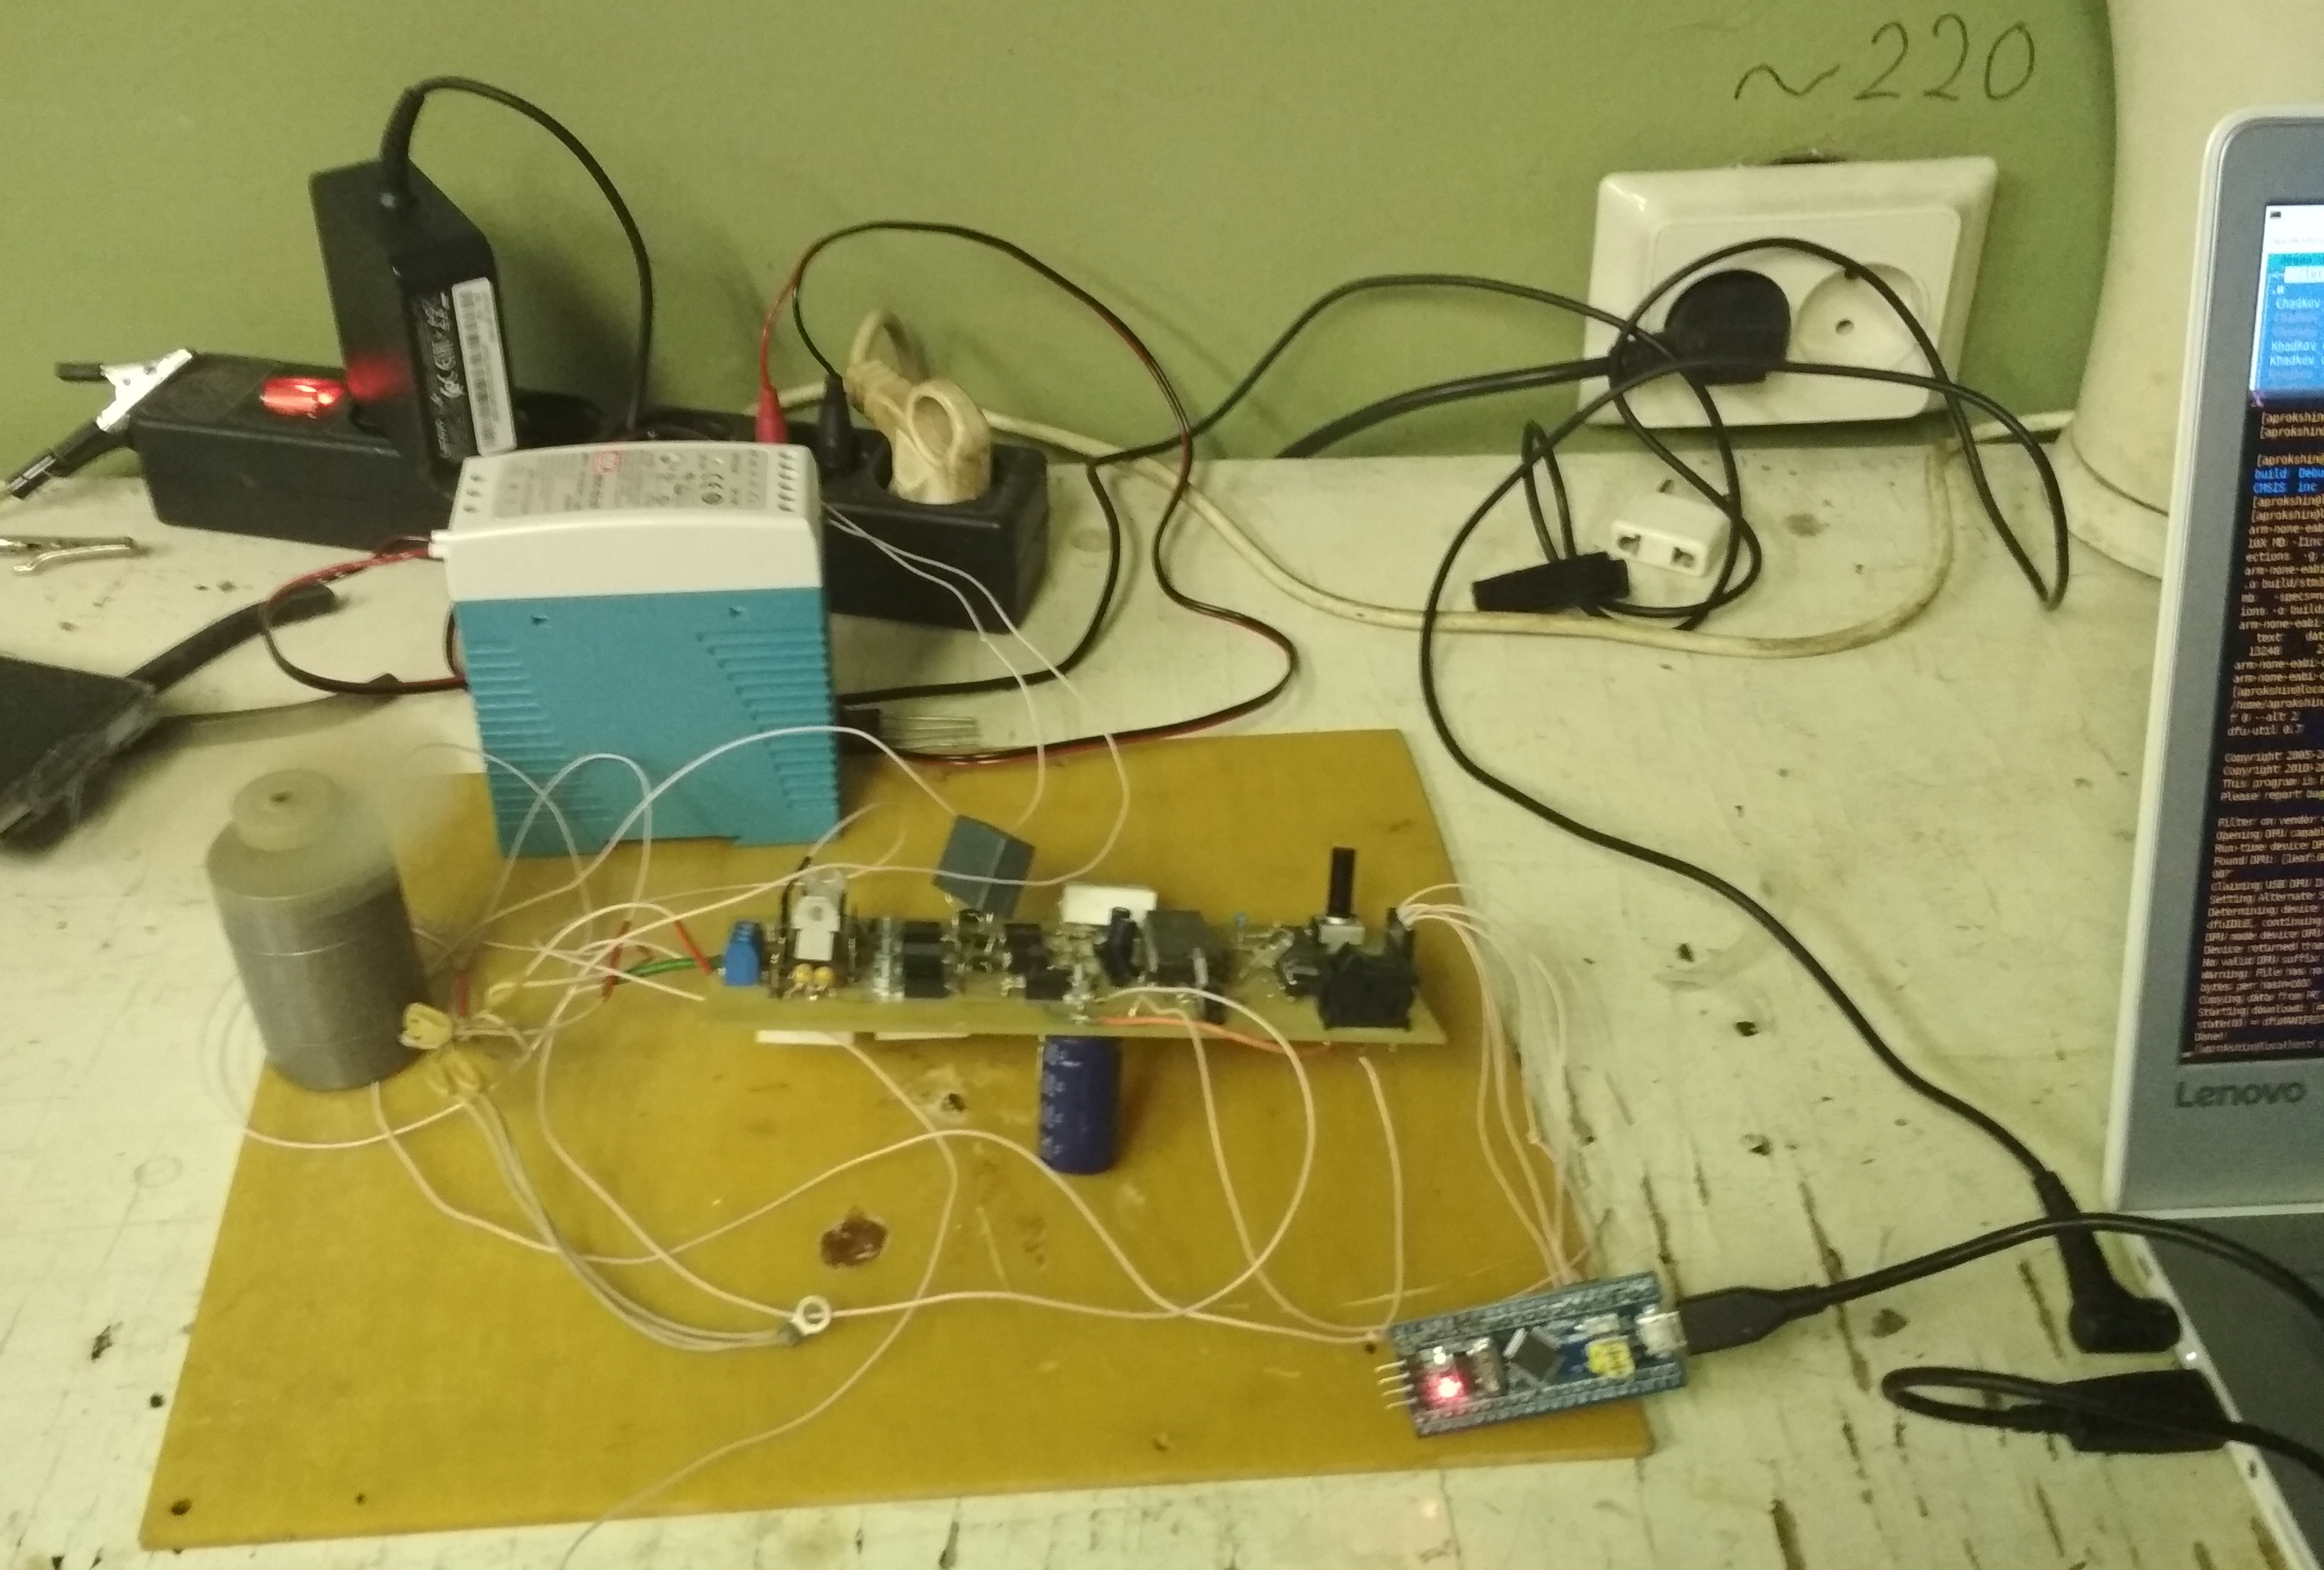
\includegraphics[width=1\linewidth]{ustanovka.jpg}}  \\
%\end{minipage}
\end{center}
\end{figure}

\end{frame}

\end{document}

